\section{15. Juni 2015}

\question{Elektronenkonfiguration von \ch{B2} ($Z=5$)}
\label{q:31}

\[\ch{B_2} : (1\sigma_g)^2 ~ (1\sigma_u^*)^2 ~ (2\sigma_g)^2 ~ (2\sigma_u^*)^2 ~ (1\pi_u)^2\]

\begin{figure}[H]
    \centering
    \begin{samepage}
        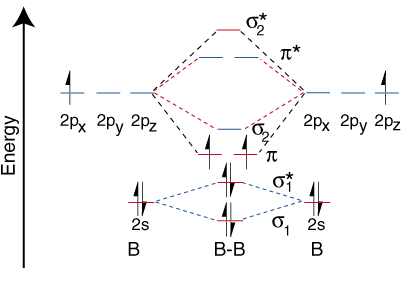
\includegraphics[width=0.8\linewidth]{resources/15-06-2015/b2.PNG}
        \caption{Elektronenkonfiguration von \ch{B2}}
    \end{samepage}
\end{figure}

\question{Arten von Para-Diamagnetismus}
\label{q:32}

\question{Konzept von Bravais-Gitter und Wigner-Seitz-Zelle}
\label{q:33}

Die Wigner-Seitz-Zelle ist definiert als die Zelle im Raum, die jedem Gitterpunkt am nächsten 
liegt. Sie hat die folgenden Eigenschaften:
\begin{enumerate}
    \item Symmetrie: Die Zelle ist symmetrisch um den Gitterpunkt, von dem aus sie konstruiert wurde, sie weist alles Symmetrieoperationen, welche im gesamten Gitter vorkommen, auf. 
    \item Ein Gitterpunkt pro Zelle: Die Zelle enthält genau einen Gitterpunkt im Inneren der Zelle. Alle anderen Gitterpunkte des Gitters liegen auf den Seitenflächen der Zelle.
    \item Nächste Nachbarn: Die Zelle teilt den Raum so auf, dass jeder Gitterpunkt seinem nächstgelegenen Nachbarn am nächsten ist. %TODO: Zirkelschluss auflösen
\end{enumerate}
Wigner-Seitz-Zelle im reziproken Raum = 1. Brillouin-Zone.

Konstruktion siehe \autoref{fig:wigner-seitz}.
\begin{figure}[H]
    \centering
    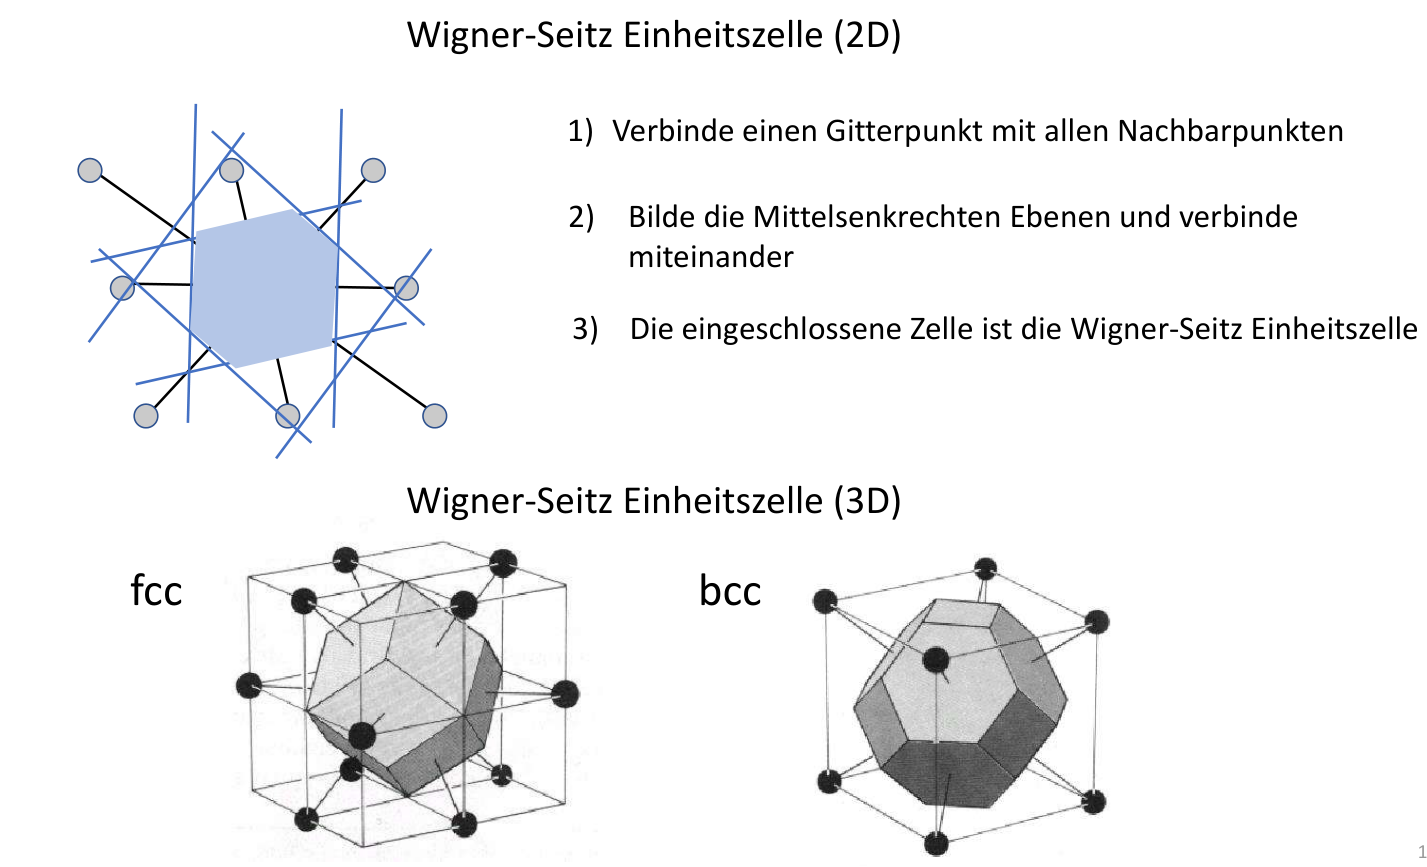
\includegraphics[width=0.8\linewidth]{resources/15-06-2015/q33.png}
    \caption{Konstruktion der Wigner-Seitz-Zelle}
    \label{fig:wigner-seitz}
\end{figure}

\question{Sp sp2 sp3 Bindungen von mehratomigen Molekülen}
\label{q:34}

Siehe \aqref{62}.

\question{Debye-Petit (oder so, irgendwas mit spezifischer Wärme von Elektronen)}
\label{q:35}

Siehe \aqref{57}.

\question{Atom-/Struktur-Faktor}
\label{q:36}

Siehe \aqref{27}.

\question{Zustandekommen von Energiebändern und Bandlücken}
\label{q:37}

\textbf{TL;DR} Braggreflexion ist die Ursache für Energiebandlücken, da bei Braggreflexion keine wellenartigen Lösungen der Schrödingergleichung existieren.
Energiebänder sind die Resultate der Energiebandlücken.

\textbf{TS;WR} Freie $e^-$ mit kontinuierlichen Energien besitzen Wellenfunktionen von der Form $\psi_{k}(\vec{r}) = \exp(i\vec{k}\vec{r})$ (ebene Welle).

Man nehme einen eindimensionalen Kristall mit Gitterkonstante $a$.
Die Braggbedingung\\$\left(\vec{k} + \vec{G}\right)^2 = k^2$ für Beugung eines Wellenvektors $\vec{k}$ ergibt sich in 1D zu
\begin{equation}
    k = \frac{\pm G}{2} = \frac{\pm n \pi}{a}
\end{equation}
wobei $G = 2\pi n/a$ ein reziproker Gittervektor ist und $n \in \mathbb{N}$.

Bei solchen $k$ (hier mit $n=1$) überlagert sich die Wellenfunktion $\exp(\pm i \pi x / a)$ eines Wandernden $e^-$ mit seiner Bragg-Reflektierten.
Mit $\exp(\pm i \pi x / a) = \cos(\pi x/a) \pm i \sin(\pi x/a)$ erhält man eine symmetrische stehende Welle
\begin{equation}
    \psi(+) = \exp( i \pi x / a) + \exp(- i \pi x / a) = 2\cos(\pi x/a)
\end{equation}
und eine antisymmetrische
\begin{equation}
    \psi(-) = \exp( i \pi x / a) - \exp(- i \pi x / a) = 2 i \sin(\pi x/a)
\end{equation}
ähnlich wie in den Hybridisierungsorbitalen einer Doppelbindung.
Die Aufenthaltswahrscheinlichkeiten $\left|\psi(\pm)\right|^2$ in Kombination mit den Potentialen der Atomkerne (Abb. (a)) zeigen, dass die symmetrische Wellenfunktion $\psi(+)$ mehr negative Ladung an die positiven Ionen zieht und dadurch geringere potentielle Energie besitzt, als eine laufende Welle und $\psi(-)$ eine höhere potentielle Energie als eine laufende Welle besitzt.
\begin{figure}[H]
    \centering
    \begin{subfigure}[c]{0.4\textwidth}
        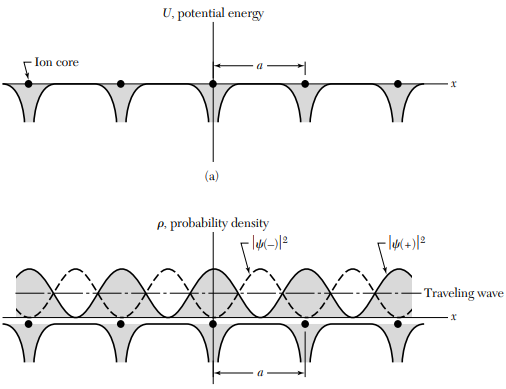
\includegraphics[width=\linewidth]{resources/15-06-2015/q37a.png}
        \caption{}
    \end{subfigure}%
    \begin{subfigure}[c]{0.4\textwidth}
        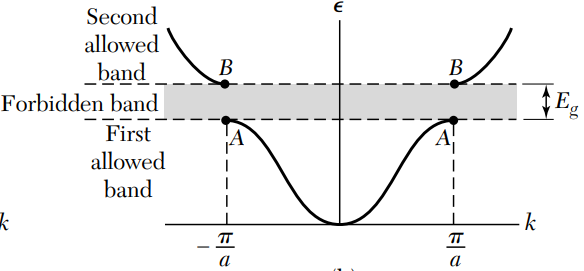
\includegraphics[width=\textwidth]{resources/15-06-2015/q37b.png}
        \caption{}
    \end{subfigure}% 
    \caption{
        (a) Aufenthaltswahrscheinlichkeiten $\left|\psi(\pm)\right|^2$ und für laufende Wellen zusammen mit der Potentiellen Energie einer negativen Ladung um die Kerne.
        (b) Energie plot mit Bandlücke.
        }
\end{figure}

\question{Zusammenhang zwischen Gitterebene und Vektoren im reziproken Gitter}
\label{q:38}

Siehe \aqref{4}.

\question{Statische Abschirmung des Elektronengases}
\label{q:39}
\textit{Annahme: Es geht um Metalle und damit um die Näherung fast freier $e^-$.}\\
Grundlage ist das Verhalten des Elektronengases um eine positive Punktladung.
Das Coloumbpotential der Punktladung müsste normal mit $r^-1$ abfallen und weitreichende Auswirkungen auf die freien $e^-$ haben:
\begin{equation*}
    \Phi_0(\vec{r}) = \frac{1}{4 \pi \epsilon_0}\frac{q}{r}
\end{equation*}
Allerdings steigt die Elektronendichte $n(\vec{r})$ um $q$ an und schwächt somit das Coloumbpotential der positiven Punktladung ab.
Das Ergebnis ist eine viel weniger weitreichendes Potential welches nur für $e^-$ in der Nähe der positiven Puntladung relevant ist.
Mathematisch kann dies durch die Thomas-Fermi(für niedrige $T$) und Debye-Hückel (für hohe $T$) Approximationen realisiert werden (siehe Wikipedia Electric-Field screening).
Dabei ergibt sich folgendes abgeschirmtes Potential:
\begin{equation*}
    \Phi(\vec{r}) = \frac{1}{4 \pi \epsilon_0}\frac{q}{r} e^{-r / r_{TF}}
\end{equation*}
Dabei ist der exponentiale Faktor die Dämpfung die durch Abschirmung entsteht und die reichweite der Coloumbwechselwirkung verringert.
$r_{TF}$ ist der Thomas-Fermi (Abschirm-) Radius.
\begin{figure}[H]
    \centering
    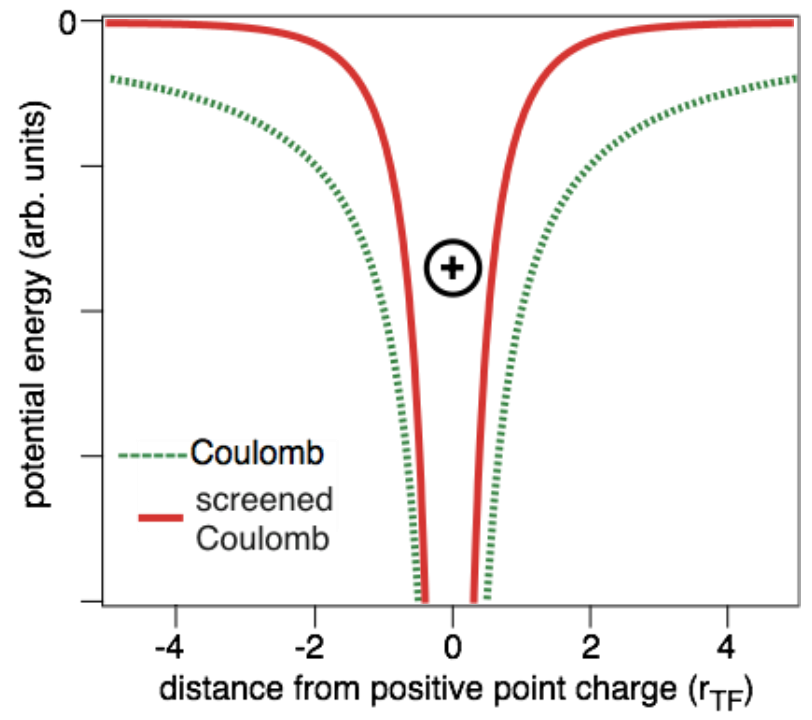
\includegraphics[width=0.3\linewidth]{resources/15-06-2015/q39_pot.png}
\end{figure}
\noindent
Diese Abschirmung führt zusammen mit der Tatsache, dass die Coloumbwechselwirkung der positiv geladenen Ionen in einem periodischen Kristallgitter zusätzlich von der Pauliwechselwirkung abgeschwächt wird, zum Modell der fast freien $e^-$
(PS.: Pauliwechselwirkung ist das abstoßen der $e^-$ vom Atomrumpf, weil dort schon Rumpfelektronen die verfügbaren Orbitale besetzen.)
\question{Einstein-Debye Unterschiede und falsche Annahmen}
\label{q:40}

\textbf{Einstein-Näherung:} 
\begin{itemize}
    \item Annahme: alle Atome im Kristall schwingen mit der gleichen Frequenz $\omega = \omega_E$, wobei $\omega_E$ die Frequenz der optischen Moden darstellt. 
    \item lässt sich nur auf optische Moden anwenden (nicht auf akustische!)
    \item funktioniert gut bei hoher Dichte der optischen Phononen und liefert richtiges 
    Hochtemperaturlimit nach Dulong-Petit-Gesetz
    \item funktioniert schlecht bei tiefen Temperaturen und liefert ungenaues Limit für niedrige Temperaturen
    \item Falsche Annahme: akustische Moden werden nicht berücksichtigt und alle harmonischen Oszillatoren im Festkörper würden mit einheitlicher Frequenz schwingen.
\end{itemize}

\textbf{Debye-Näherung:} 
\begin{itemize}
    \item Annahme: 
        \begin{itemize}
            \item Vielzahl möglicher Frequenzen und Ausbreitungsgeschwindigkeit $v_i$ von Wellen/Phononen. 
            \item Lineare Dispersion $\omega_i=v_ik$ 
        \end{itemize}
    \item berücksichtigt nur akustische Moden
    \item funktioniert gut bei niedrigen Temperaturen, da niederenergetische (akustische) Phononen besser dargestellt sind 
    \item liefert korrektes Limit für hohe und tiefe Temperaturen
    \item Falsche Annahme: optische Phononen werden nicht berücksichtigt und Effekte nahe der Brillouinzonengrenze werden nicht richtig beschrieben
\end{itemize}

\begin{figure}[H]
    \centering
    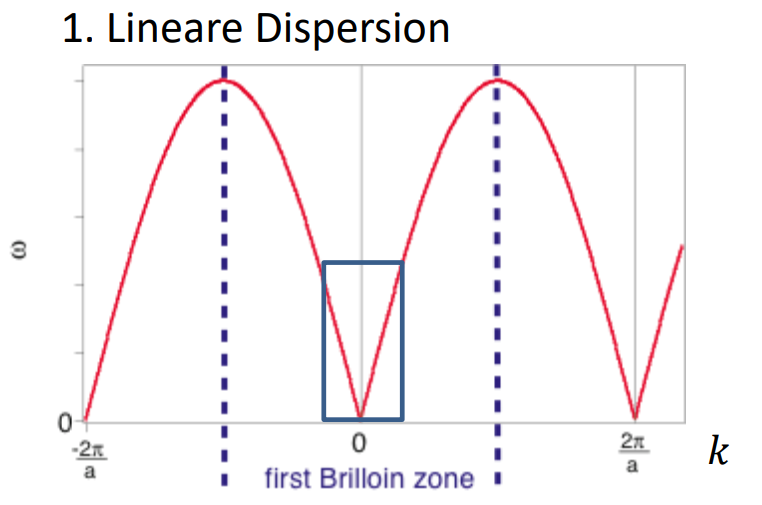
\includegraphics[width=0.6\textwidth]{resources/15-06-2015/debye_dispersion.png}
    \caption{Debye linearer Zusammenhang nur in blauen Kastl gerechtfertigt. Nicht an Brillouinzonengrenze.}
    %\label{}
   \end{figure}

\begin{figure}[H]
 \centering
 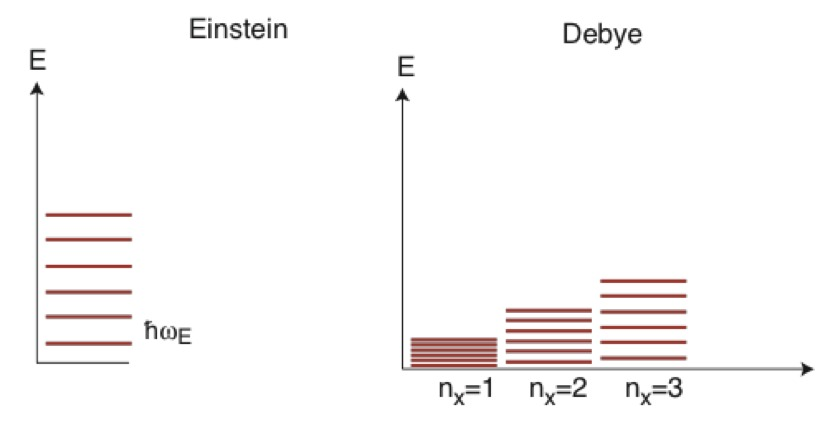
\includegraphics[width=0.6\textwidth]{resources/15-06-2015/Einstein_Debye.jpeg}
 \caption{Einstein- vs. Debye-Modell}
 %\label{}
\end{figure}
\newpage